\begin{comment}
    \begin{itemize}
        \item Unified discussion of results
        \item How they reinforce or contrast eachother
    \end{itemize}
\end{comment}

\subsection{Simulation Study}
To validate the variational model, we conduct a simulation study.
    As the problem of multivariate extremes is the estimation of the dependence
    structure of the extremes, we focus the simulation study on on estimation of
    the angular distribution.  The simulated data is generated from a finite
    mixture of projected gammas, at varying levels of dimensionality and number
    of mixture components.  For each simulation, for a \emph{training} dataset,
    \num{1000} replicates are sampled.  For each simulation, for a 
    \emph{testing} dataset, another \num{1000} replicates are sampled using
    the same distributional parameters.

To evaluate the fidelity of the variational implementation as compared to MCMC, 
    we use a the \emph{energy score} criterion \citep{gneiting2007}, which is a
    generalization of the \emph{continuous ranked probability score} to a
    multivariate setting.  This energy score criterion takes the form
    \[
      S_{\text{ES}}(P, \bm{x}) = \text{E}_p\left[g(\bm{X},\bm{x})\right] - 
        \frac{1}{2}\text{E}_p\left[g(\bm{X},\bm{X}^{\prime})\right]
    \]
    where $g$ is a kernel function, $\bm{x}$ is an observed value, and 
    $\bm{X},\bm{X}^{\prime}$ are posterior predictive replicates of $\bm{x}$.
    When energy score is used with an appropriate negative definite kernel 
    metric, it forms a \emph{proper} scoring rule. The specific negative 
    definite kernel we use is described in Prop.~3 of \cite{trubey:pg}.  Though 
    geodesic distance on $\mathbb{S}_{\infty}^{d-1}$ is computationally inefficient,
    for points on two different faces of $\mathbb{S}_{\infty}^{d-1}$,
    they find a computationally efficient upper bound on geodesic distance by 
    remembering that all faces are pairwise adjacent, and rotating one face into the
    same hyperplane as the other.  Then the kernel metric is the Euclidean distance
    between the first point, and the rotated second point.
    
    In Figure~\ref{fig:energyscore} we compare rise in energy score of the fitted
    model over a \emph{baseline} energy score.  This baseline energy score is so
    named because it is the energy score between a target dataset and another
    dataset from the same generating distribution.  A value of 0 is optimal.
    \makenote{add additional model for comparison}  Note displayed scores are 
    averaged over 10 iterations \makenote{rewrite}.
    
    We see some minor loss in fidelity for the variational model as compared to 
    the MCMC model as is expected from the variational approximation.  With that
    said, the variational approximation is still quite good.

\subsection{SLOSH}
\subsubsection{Delaware Bay}

\begin{figure}[ht]
    \caption{Locations of identified sites that experienced inundation in more than 
        $5$ percent of storms.  Specifically identified are two locations of 
        interest. \makenote{Change Label to PIA} \label{map:delawarebay}}
    \centering
    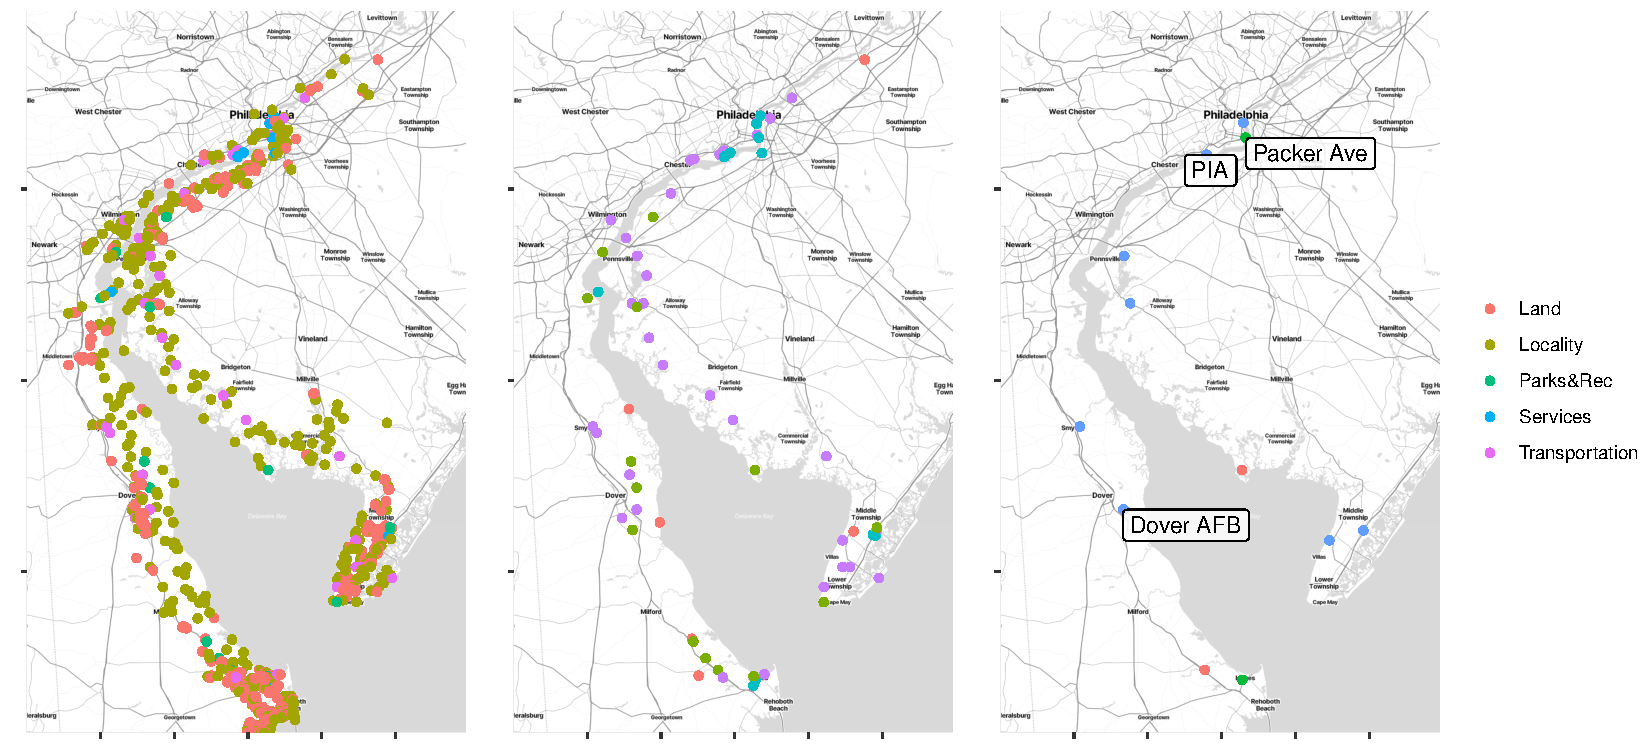
\includegraphics[height=4in]{./plots/delaware}
\end{figure}

The range of latitudes at which storms make landfall in the simulation cover a region of
    coastline surrounding the entrance of Delaware Bay \makenote{rephrase more accurate given
    data}.  Given that focus inherent in the original data, we focus our primary analysis there.
    Intersecting the original \emph{SLOSH} grid for the Delaware bay and surrounding watershed, 
    for grid cells that experienced inundation in more than 5 percent of simulations, 
    with specified locations, we identify 65 locations of interest, at which we will conduct 
    our analysis.  Figure~\ref{map:delawarebay} gives the locations of sites we identified, along
    with a classification of those sites.  Services includes emergency services, police, fire,
    and medical services.  Land includes village centers, major intersections, and named
    land features.  Transportation includes ferry landings, airports, heliports, and similar.
    Within that set, we further identify two locations of particular interest, 
    for which significant inundation can lead to catastrophic consequences:  
    Dover Air Force Base (Dover AFB), and the Philadelphia International 
    Airport (PIA). Dover AFB is situated next to Delaware Bay, with a direct approach from the
    open ocean.  PIA, on the other hand, is further upstream, adjacent to the Delaware River, 
    in the city of Philadelphia.  To reach this location, storm surge would need to backflow 
    the Delaware River a significant distance.

One difficulty with a high-dimensional model is evaluating its fidelity.  As we saw in the simulation
    study, the relative rise in energy score between a bad model and a good model shrinks as
    dimensionality increases.  This is related to the curse of dimensionality in applications like
    $k$-nearest neighbor algorithms: as the number of dimensions increases, the ratio in average
    distance between the nearest replicate, and farthest replicate in a sample will tend to approach 1.
    So distance as a measure is fundamentally flawed in a high-dimensional setting.

One thing we can do is evaluate recovery of marginal empirical CDF's, using marginal
    predictive CDF's.  In Figure~\ref{plot:marginal_doverafb}, we plot the marginal
    empirical CDF relative to the posterior predictive CDF under \num{4} models.  
    Having sampled $\bm{V}^{*}$ from its posterior predictive density, we can get a sample of $W_s^*$
    by inverting Equation~\eqref{eqn:standardization}---accepting the inevitable truncation.  Thus
    for $R^*\sim\text{Pareto}(1)$, $Z^* = R^*\bm{V}^*$,
    \begin{equation*}
        W_s^* = a_s\left(\frac{(Z_s^*)^{\xi_s} - 1}{\xi_s}\right) + b_s
    \end{equation*}
    where $\bm{\xi}$, $\bm{a}$, and $\bm{b}$ were previously calculated.  
    
    
    
    
    We observe here that 
    the recovery of the marginal CDF is somewhat problematic for the Variational Bayes
    approach. 


To evaluate the efficacy of our models in a moderately high-dimensional setting,
    we evaluate their recovery of their marginal distributions.  In 
    Figures~\ref{plot:marginal_doverafb},\ref{plot:marginal_pia} we observe the marginal 
    cumulative distribution functions for $\bm{V}$ and $\bm{Z}$ at Dover AFB and PIA,
    as calculated from from the posterior predictive distribution.  Note, in particular,
    that the variational model experiences significant difficulty in recovering the
    CDF from the original data.  Fitting via MCMC comes closest to the target.
    
\begin{figure}[ht]
    \caption{Recovery of marginal $\bm{v}$ (left) and $\bm{z}$ (right) for 
        Dover Air Force Base.\makenote{Change Z to W, to reflect reality.}
        \label{plot:marginal_doverafb}}
    \centering
    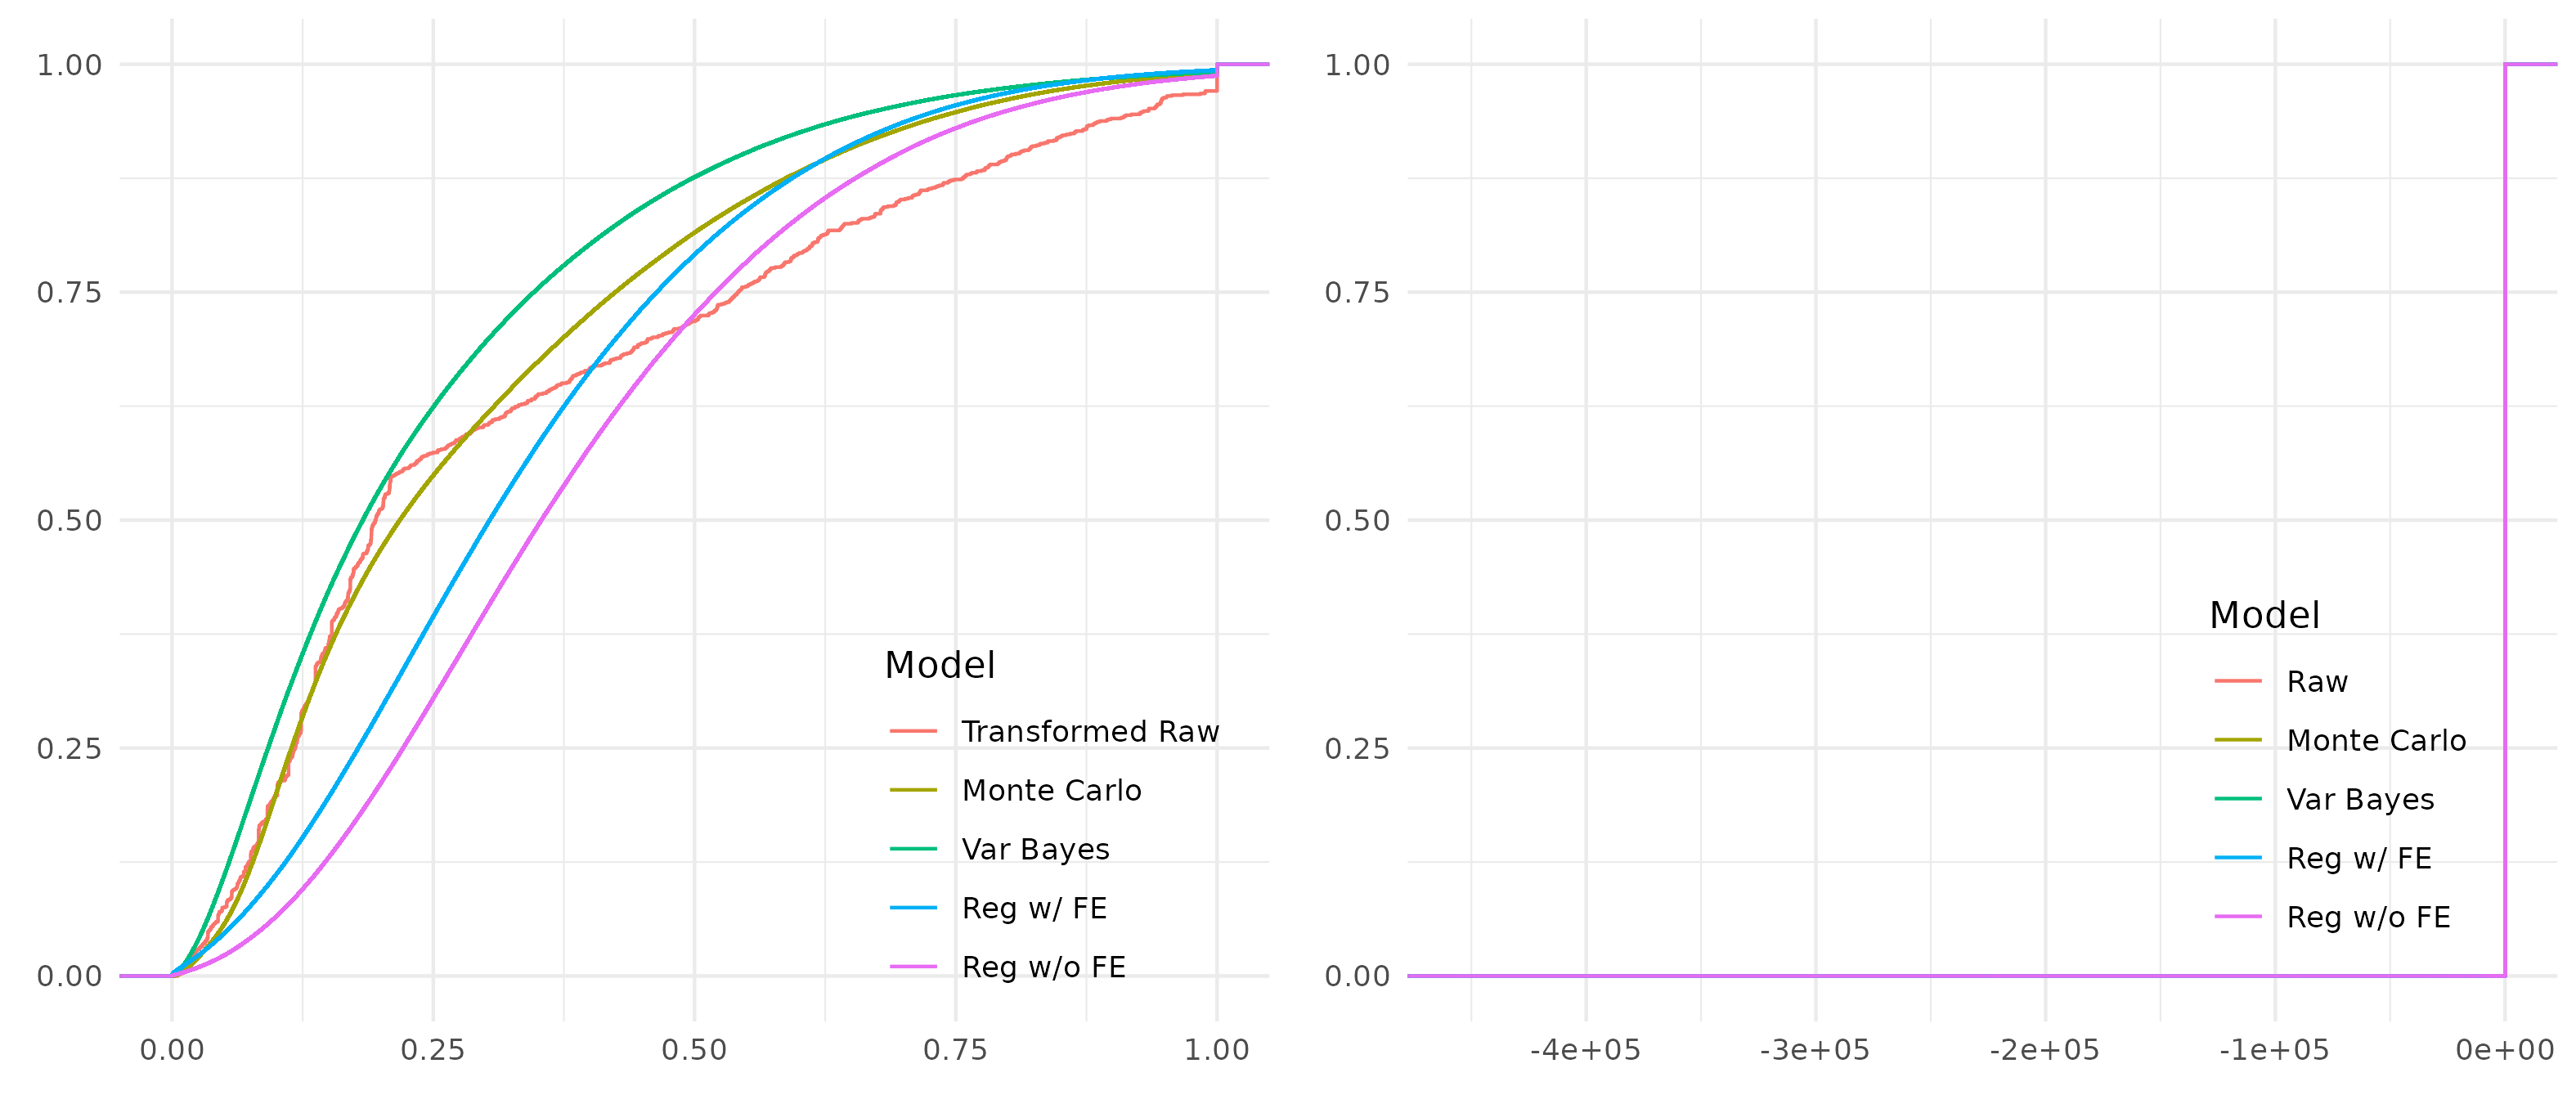
\includegraphics[width=\textwidth]{./plots/delaware_marginal_dover_afb}
\end{figure}










\begin{figure}[ht]
    \caption{Recovery of marginal $\bm{v}$ (left) and $\bm{z}$ (right) for 
        Philadelphia International Airport.\makenote{Change Z to W, to reflect reality.}
        \label{plot:marginal_pia}}
    \centering
    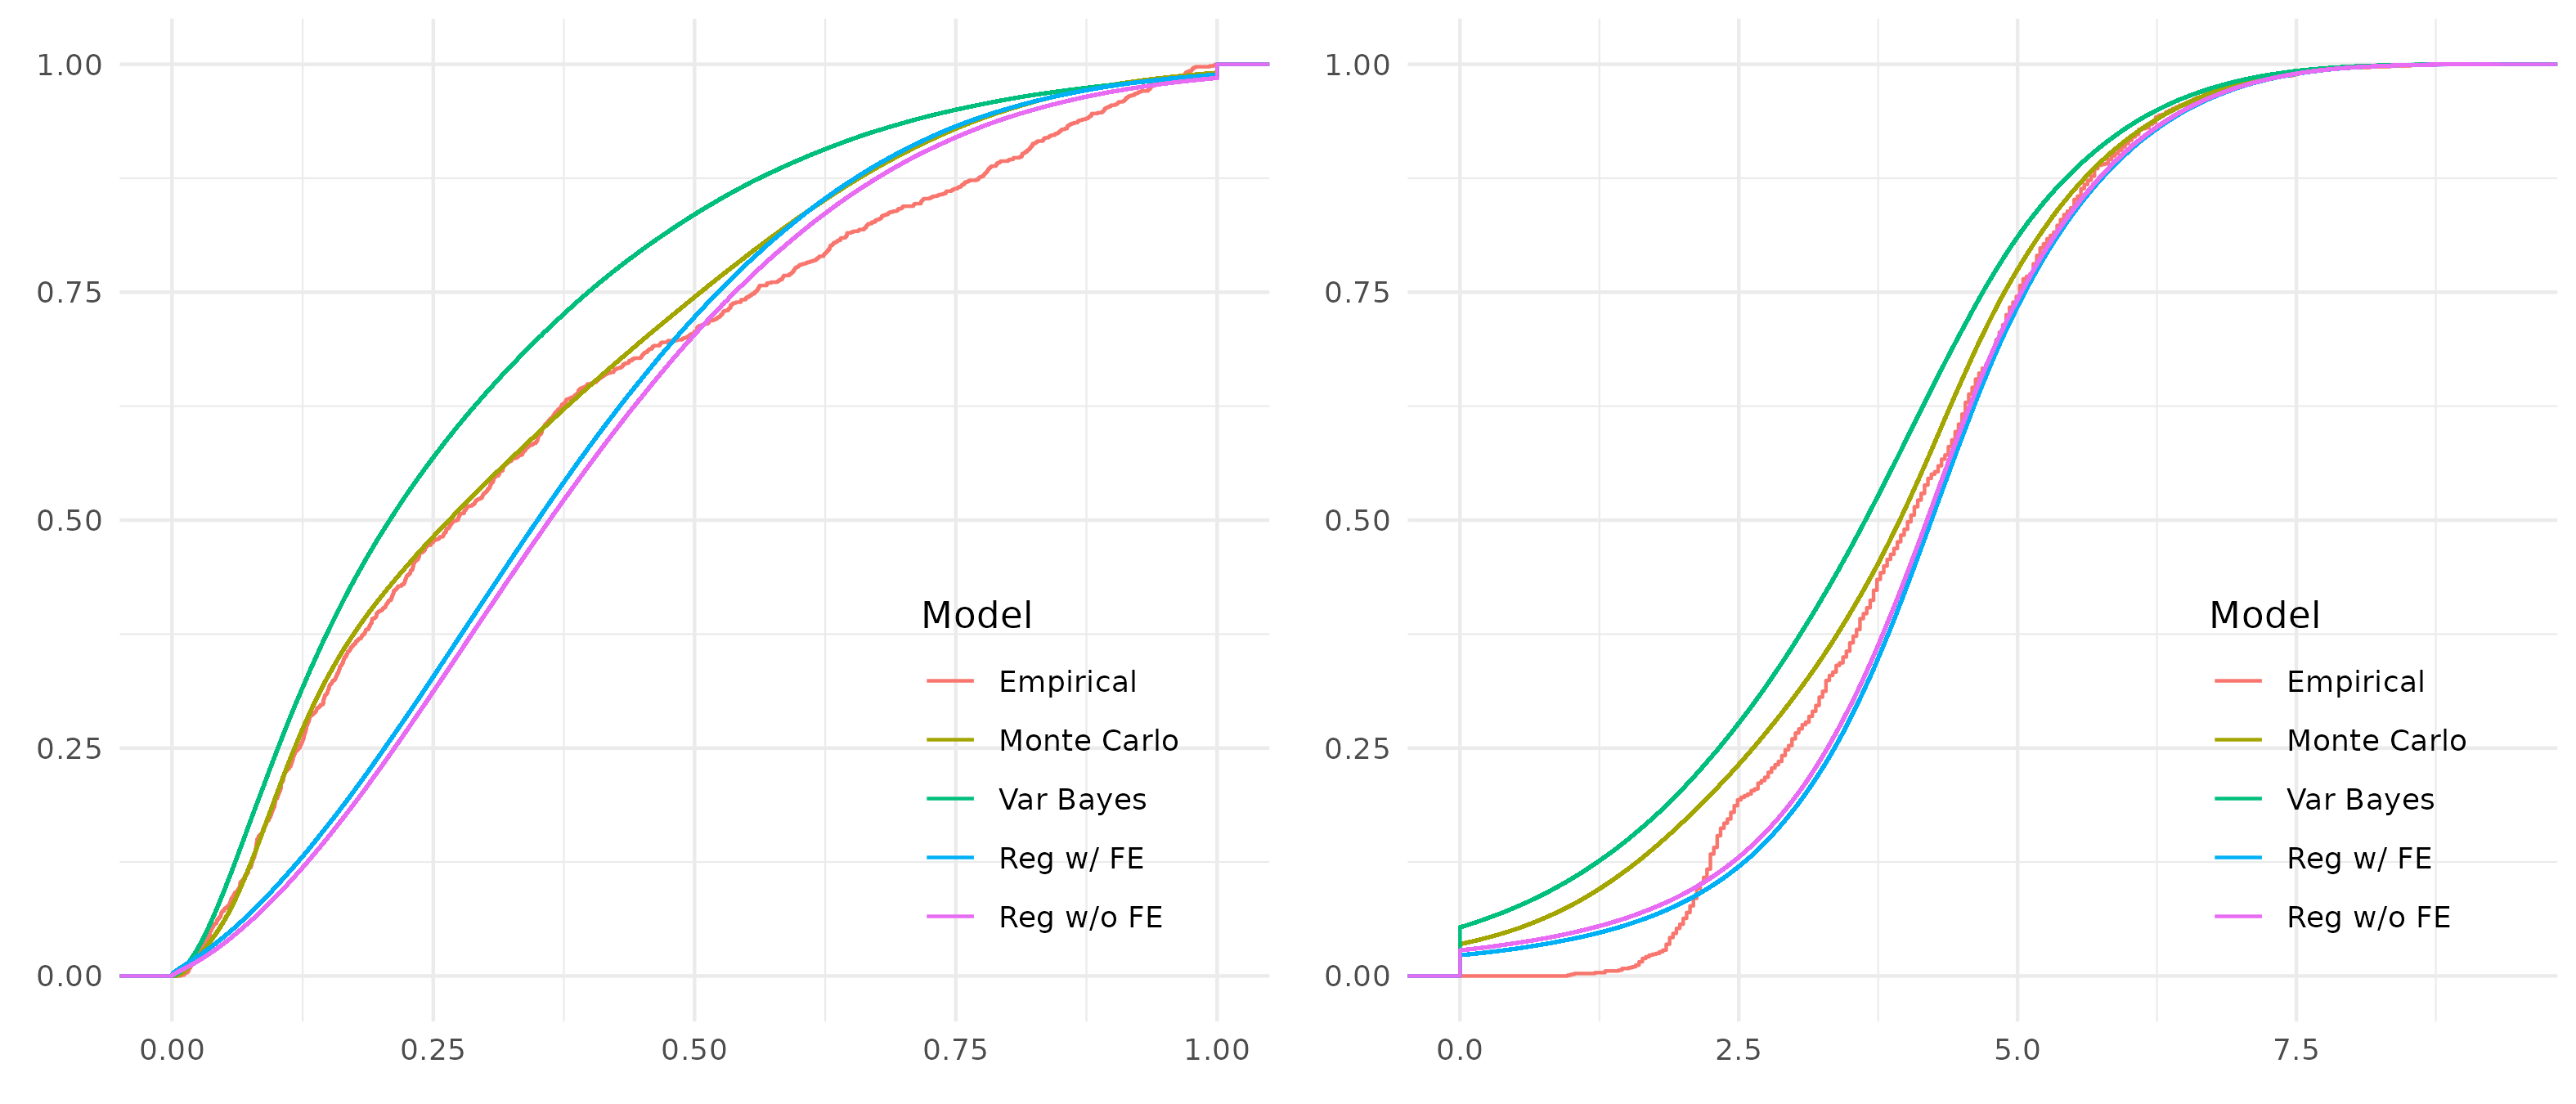
\includegraphics[width=\textwidth]{./plots/delaware_marginal_phil_ia}
\end{figure}
% EOF